To provide a comprehensive and representative view, the tests are structured into five subsections, each corresponding to a different Ethernet frame size. 
Four of the selected sizes -- 64 bytes, 512 bytes, 1280 bytes, and 1518 bytes -- are recommended by RFC~2544~\cite{rfc2544} 
covering both edge cases and practically relevant intermediate values. 
The fifth size, 889 bytes, was chosen based on real-world traffic analysis by Jurkiewicz et al.~\cite{JURKIEWICZ202115}, who identified it as the average frame size observed in modern network environment.
This selection covers the full range of standard Ethernet frame sizes, from the minimum to the maximum non-jumbo frames, 
while also including a statistically representative average.

All tests were conducted at four different transmission speeds -- 1, 10, 25, and 40 Gbit/s -- to evaluate the behavior of each configuration under varying network loads.

Traffic in all scenarios is generated using TRex with the TBD profile,
which ensures that each packet carries a unique source IP address to simulate multiple concurrent clients, while maintaining a single destination IP per direction.
Since the aim of this thesis is to evaluate the VPP architecture rather than specific features (e.g., routing table lookup or hashing mechanisms),
the routing table of the DUT contains only two active forwarding entries corresponding to the test routes,
along with two administrative entries used for management purposes.

The DUT is configured with the VPP stack and tested under three levels of parallelism: using 1, 4, and 10 worker threads, plus a single main thread in all configurations.
The worker threads are pinned to the NUMA node closest to the NICs to minimize memory access latency.
The number of RX/TX queues is aligned with the number of active worker threads in each configuration to ensure balanced packet distribution and optimal resource utilization.

To provide a baseline for comparison, all scenarios are also executed using the standard Linux kernel networking stack.
It is configured with routing and interface parameters equivalent to the VPP setup, utilizing all 10 CPU cores on the NUMA node closest to the NICs.
RPS is enabled, with affinities set evenly across the cores.
This allows for a direct comparison between VPP and traditional kernel-based forwarding in terms of performance and energy efficiency.

\subsection{One-way forwarding}

These tests were conducted in a one-way configuration, as suggested by RFC2544\cite{rfc2544}.
This scenario can simulate networks with asymmetric traffic patterns (e.g., an HTTP server) or reflect conditions similar to a DoS attack.

%----------------------------------
\subsubsection{1 Gbps Test Results}

\begin{table}[h!]
\centering
\caption{Results of one-way 1 Gbit/s of 64-byte frames}
\begin{tabular}{|l|r|r|r|r|r|r|}
\hline
\multicolumn{1}{|c|}{\textbf{Config}} &
\multicolumn{1}{c|}{\textbf{Energy [Wh] }} &
\multicolumn{1}{c|}{\textbf{Pkt Loss [\%]}} &
\multicolumn{1}{c|}{\textbf{Avg Lat [$\mu$s]}} &
\multicolumn{1}{c|}{\textbf{Jitter [$\mu$s]}} \\
\hline 
VPP-1 & 5.68 & 0.00 & 12.8 & 9.5 \\
VPP-4 & 6.46 & 0.00 & 27.45 & 13.55 \\
VPP-10 & 7.86 & 0.00 & 28.3 & 12.65 \\
Linux & 6.78 & 0.00 & 108.05 & 97.25 \\
\hline
\end{tabular}
\label{tab:1udp:64B}
\end{table}


%------------------------------------------------------
\begin{table}[h!]
\centering
\caption{Results of one-way 1 Gbit/s of 512-byte frames}
\begin{tabular}{|l|r|r|r|r|r|r|}
\hline
\multicolumn{1}{|c|}{\textbf{Config}} &
\multicolumn{1}{c|}{\textbf{Energy [Wh] }} &
\multicolumn{1}{c|}{\textbf{Pkt Loss [\%]}} &
\multicolumn{1}{c|}{\textbf{Avg Lat [$\mu$s]}} &
\multicolumn{1}{c|}{\textbf{Jitter [$\mu$s]}} \\
\hline 
VPP-1 & 5,69 & 0.00 & 12.1 & 11.7 \\
VPP-4 & 6.48 & 0.00 & 22.85 & 17.4 \\
VPP-10 & TODO &  &  &  \\
Linux & 6.23 & 0.00 & 56.1 & 51.35 \\
\hline
\end{tabular}
\label{tab:1udp:512B}
\end{table}


%------------------------------------------------------
\begin{table}[h!]
\centering
\caption{Results of one-way 1 Gbit/s of 889-byte frames}
\begin{tabular}{|l|r|r|r|r|r|r|}
\hline
\multicolumn{1}{|c|}{\textbf{Config}} &
\multicolumn{1}{c|}{\textbf{Energy [Wh] }} &
\multicolumn{1}{c|}{\textbf{Pkt Loss [\%]}} &
\multicolumn{1}{c|}{\textbf{Avg Lat [$\mu$s]}} &
\multicolumn{1}{c|}{\textbf{Jitter [$\mu$s]}} \\
\hline 
VPP-1 & 5,76 & 0.00 & 10.3 & 8.4 \\
VPP-4 & 6.45 & 0.00 & 21.3 & 17.6 \\
VPP-10 & 7.85 & 0.00 & 20.95 & 16.3  \\
Linux & TODO &  &  &  \\
\hline
\end{tabular}
\label{tab:1udp:889B}
\end{table}


%------------------------------------------------------
\begin{table}[h!]
\centering
\caption{Results of one-way 1 Gbit/s of 1280-byte frames}
\begin{tabular}{|l|r|r|r|r|r|r|}
\hline
\multicolumn{1}{|c|}{\textbf{Config}} &
\multicolumn{1}{c|}{\textbf{Energy [Wh] }} &
\multicolumn{1}{c|}{\textbf{Pkt Loss [\%]}} &
\multicolumn{1}{c|}{\textbf{Avg Lat [$\mu$s]}} &
\multicolumn{1}{c|}{\textbf{Jitter [$\mu$s]}} \\
\hline 
VPP-1 & TODO &  &  &  \\
VPP-4 & 6.46 & 0.00 & 18.3 & 17.2 \\
VPP-10 & 7.84 & 0.00 & 18.8 & 15.95  \\
Linux & TODO &  &  &  \\
\hline
\end{tabular}
\label{tab:1udp:1280B}
\end{table}


%------------------------------------------------------
\begin{table}[h!]
\centering
\caption{Results of one-way 1 Gbit/s of 1518-byte frames}
\begin{tabular}{|l|r|r|r|r|r|r|}
\hline
\multicolumn{1}{|c|}{\textbf{Config}} &
\multicolumn{1}{c|}{\textbf{Energy [Wh] }} &
\multicolumn{1}{c|}{\textbf{Pkt Loss [\%]}} &
\multicolumn{1}{c|}{\textbf{Avg Lat [$\mu$s]}} &
\multicolumn{1}{c|}{\textbf{Jitter [$\mu$s]}} \\
\hline 
VPP-1 & 5.66 & 0.00 & 7.2 & 5.5  \\
VPP-4 & 6.42 & 0.00 & 16.1 & 15.75 \\
VPP-10 & 7.84 & 0.00 & 18.8 & 15.95 \\
Linux & TODO &  &  &  \\
\hline
\end{tabular}
\label{tab:1udp:1518B}
\end{table}

%---------------------------------------------------------------------------------------------
%---------------------------------------------------------------------------------------------
%---------------------------------------------------------------------------------------------
\subsubsection{10 Gbps Test Results}

As shown in Tab.~\ref{tab:10udp:64B}, both VPP-1 and the Linux stack were unable to handle this packet rate at 10~Gbit/s with 64-byte frames, resulting in high packet loss and significantly increased latency. 
VPP-4 managed to process the traffic with minimal loss, achieving the lowest latency and jitter among all configurations. 
VPP-10 also completed the test losslessly, but with slightly higher latency. 

%------------------------------------------------------
\begin{table}[h!]
\centering
\caption{Results of one-way 10 Gbit/s of 64-byte frames}
\begin{tabular}{|l|r|r|r|r|r|r|}
\hline
\multicolumn{1}{|c|}{\textbf{Config}} &
\multicolumn{1}{c|}{\textbf{Energy [Wh] }} &
\multicolumn{1}{c|}{\textbf{Pkt Loss [\%]}} &
\multicolumn{1}{c|}{\textbf{Avg Lat [$\mu$s]}} &
\multicolumn{1}{c|}{\textbf{Jitter [$\mu$s]}} \\
\hline 
VPP-1 & 5.72 & 59.5 & 589.50 & 14.05 \\
VPP-4 & 6.56 & 0.02 & 20.60 & 6.00 \\
VPP-10 & 8.04 & 0.00 & 30.00 & 12.90 \\
Linux & 7.35 & 80.97 & 3846.30 & 217.8 \\
\hline
\end{tabular}
\label{tab:10udp:64B}
\end{table}

It can be seen from Tab.~\ref{tab:10udp:512B} that increasing the frame size to 512~bytes allowed all tested configurations to handle the traffic without packet loss. 
Although the latency of the Linux stack improved significantly compared to the previous measurement, it still remained the highest among all configurations.
The energy consumption of the Linux configuration decreased, likely due to reduced overhead from system calls.

%------------------------------------------------------
\begin{table}[h!]
\centering
\caption{Results of one-way 10 Gbit/s of 512-byte frames}
\begin{tabular}{|l|r|r|r|r|r|r|}
\hline
\multicolumn{1}{|c|}{\textbf{Config}} &
\multicolumn{1}{c|}{\textbf{Energy [Wh] }} &
\multicolumn{1}{c|}{\textbf{Pkt Loss [\%]}} &
\multicolumn{1}{c|}{\textbf{Avg Lat [$\mu$s]}} &
\multicolumn{1}{c|}{\textbf{Jitter [$\mu$s]}} \\
\hline 
VPP-1 & 5.60 & 0.00 & 19.95 & 12.00 \\
VPP-4 & 6.48 & 0.00 & 28.20 & 14.50 \\
VPP-10 & 7.97 & 0.00 & 29.05 & 13.65 \\
Linux & 6.85 & 0.00 & 129.4 & 99.35 \\
\hline
\end{tabular}
\label{tab:10udp:512B}
\end{table}

In this test with 889-byte frames, all VPP configurations show similar results to the previous measurement, although with slightly increased jitter.
This may be due to VPP constructing processing vectors based on the number of packets rather than their total size.
The increased frame size improved Linux's average latency, possibly due to reduced per-packet processing overhead.
The discussed results are summarized in Table~\ref{tab:10udp:889B}.

%------------------------------------------------------
\begin{table}[h!]
\centering
\caption{Results of one-way 10 Gbit/s of 889-byte frames}
\begin{tabular}{|l|r|r|r|r|r|r|}
\hline
\multicolumn{1}{|c|}{\textbf{Config}} &
\multicolumn{1}{c|}{\textbf{Energy [Wh] }} &
\multicolumn{1}{c|}{\textbf{Pkt Loss [\%]}} &
\multicolumn{1}{c|}{\textbf{Avg Lat [$\mu$s]}} &
\multicolumn{1}{c|}{\textbf{Jitter [$\mu$s]}} \\
\hline 
VPP-1 & 5.62 & 0.00 & 23.4 & 14.95 \\
VPP-4 & 6.48 & 0.00 & 26.5 & 18.25 \\
VPP-10 & 7.95 & 0.00 & 26.95 & 17.55 \\
Linux & 6.67 & 0.00 & 66.45 & 68.3 \\
\hline
\end{tabular}
\label{tab:10udp:889B}
\end{table}

As shown in Table~\ref{tab:10udp:1280B}, the VPP configurations performed similarly to the previous measurement.
In contrast, Linux achieved slightly improved latency and jitter, potentially due to the larger frame size further reducing per-packet processing overhead. 

%------------------------------------------------------
\begin{table}[h!]
\centering
\caption{Results of one-way 10 Gbit/s of 1280-byte frames}
\begin{tabular}{|l|r|r|r|r|r|r|}
\hline
\multicolumn{1}{|c|}{\textbf{Config}} &
\multicolumn{1}{c|}{\textbf{Energy [Wh] }} &
\multicolumn{1}{c|}{\textbf{Pkt Loss [\%]}} &
\multicolumn{1}{c|}{\textbf{Avg Lat [$\mu$s]}} &
\multicolumn{1}{c|}{\textbf{Jitter [$\mu$s]}} \\
\hline 
VPP-1 & 5.58 & 0.00 & 22.8 & 17.05 \\
VPP-4 & 6.47 & 0.00 & 25.95 & 16.90 \\
VPP-10 & 7.98 & 0.00 & 26.80 & 16.60 \\
Linux & 6.54 & 0.00 & 57.05 & 65.50 \\
\hline
\end{tabular}
\label{tab:10udp:1280B}
\end{table}

The results for 1518-byte frames are consistent with those observed at 1280 bytes, with no significant improvements in consumption, latency, or jitter.
This suggests that increasing the frame size beyond 1280 bytes does not bring further performance gains in the tested configurations.
The detailed results are presented in Table~\ref{tab:10udp:1518B}.

%------------------------------------------------------
\begin{table}[h!]
\centering
\caption{Results of one-way 10 Gbit/s of 1518-byte frames}
\begin{tabular}{|l|r|r|r|r|r|r|}
\hline
\multicolumn{1}{|c|}{\textbf{Config}} &
\multicolumn{1}{c|}{\textbf{Energy [Wh] }} &
\multicolumn{1}{c|}{\textbf{Pkt Loss [\%]}} &
\multicolumn{1}{c|}{\textbf{Avg Lat [$\mu$s]}} &
\multicolumn{1}{c|}{\textbf{Jitter [$\mu$s]}} \\
\hline 
VPP-1 & 5.57 & 0.00 & 20.45 & 14.95 \\
VPP-4 & 6.48 & 0.00 & 24.00 & 17.45 \\
VPP-10 & 7.97 & 0.00 & 25.40 & 17.70 \\
Linux & 6.51 & 0.00 & 61.75 & 65.80 \\
\hline
\end{tabular}
\label{tab:10udp:1518B}
\end{table}

Figure~\ref{fig:10g} shows the energy efficiency of each configuration in this test in terms of delivered packets and bytes.
The significant drop in performance for VPP-1 and Linux in 64-byte frames test is caused by large packet loss.
When all packets are successfully delivered, all VPP configurations maintain stable BPWh values, which is due to their busy-wait processing model.
The Linux stack, on the other hand, becomes more efficient with increasing frame size, likely as a result of less frequent system calls.

\begin{figure}[!htbp]
    \centering
    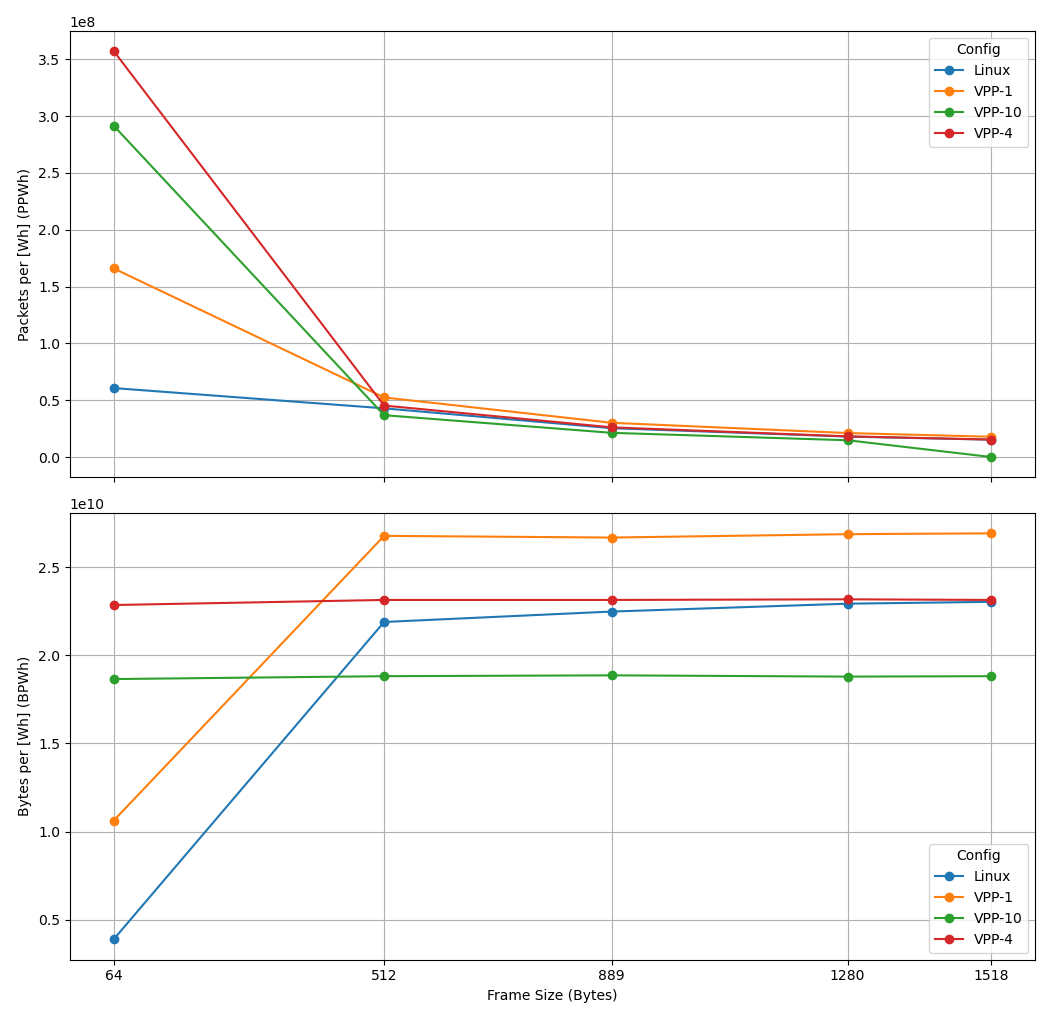
\includegraphics[width=\linewidth]{images/consumption-10g.png}
    \caption{Energy efficiency per delivered data in one-way 10\,Gbit/s.}
    \label{fig:10g}
\end{figure}



%---------------------------------------------------------------------------------------------
%---------------------------------------------------------------------------------------------
%---------------------------------------------------------------------------------------------
\subsubsection{25 Gbps Test Results}

As shown in Table~\ref{tab:25udp:64B}, none of the configurations were able to deliver all data.
In all VPP setups, the delivered data maintained low jitter,
likely due to lost packets in RX queues being overwritten by fresher incoming traffic.
This stress test also demonstrates that the Linux stack is unable to handle such network load, resulting in extremely high latency of delivered packets.
These results highlight the advantages of VPP under heavy traffic conditions.

%------------------------------------------------------
\begin{table}[h!]
\centering
\caption{Results of one-way 25 Gbit/s of 64-byte frames}
\begin{tabular}{|l|r|r|r|r|r|r|}
\hline
\multicolumn{1}{|c|}{\textbf{Config}} &
\multicolumn{1}{c|}{\textbf{Energy [Wh] }} &
\multicolumn{1}{c|}{\textbf{Pkt Loss [\%]}} &
\multicolumn{1}{c|}{\textbf{Avg Lat [$\mu$s]}} &
\multicolumn{1}{c|}{\textbf{Jitter [$\mu$s]}} \\
\hline 
VPP-1 & 5.59 & 83.29 & 577.5 & 7.70 \\
VPP-4 & 6.56 & 49.00 & 198.85 & 7.65 \\
VPP-10 & 8.26 & 29.55 & 155.35 & 11.95 \\
Linux & 7.43 & 92.71 & 5597.95 & 632.00 \\
\hline
\end{tabular}
\label{tab:25udp:64B}
\end{table}

When the frame size increased to 512 bytes, all VPP configurations were able to deliver the full traffic,
except for VPP-1, which dropped a negligible amount of packets.
All VPP setups showed reduced latency and jitter compared to the previous test.
The Linux stack, however, was still unable to handle the traffic, dropping nearly 50\% of the packets and showing extremely high latency in the delivered traffic,
as summarized in Table~\ref{tab:25udp:512B}.

%------------------------------------------------------
\begin{table}[h!]
\centering
\caption{Results of one-way 25 Gbit/s of 512-byte frames}
\begin{tabular}{|l|r|r|r|r|r|r|}
\hline
\multicolumn{1}{|c|}{\textbf{Config}} &
\multicolumn{1}{c|}{\textbf{Energy [Wh] }} &
\multicolumn{1}{c|}{\textbf{Pkt Loss [\%]}} &
\multicolumn{1}{c|}{\textbf{Avg Lat [$\mu$s]}} &
\multicolumn{1}{c|}{\textbf{Jitter [$\mu$s]}} \\
\hline 
VPP-1 & 5.57 & 0.07 & 31.85 & 11.15 \\
VPP-4 & 6.43 & 0.00 & 29.55 & 13.75 \\
VPP-10 & 8.03 & 0.00 & 31.00 & 14.45 \\
Linux & 7.57 & 47.97 & 7819.60 & 477.55 \\
\hline
\end{tabular}
\label{tab:25udp:512B}
\end{table}

As indicated by the results in Table~\ref{tab:25udp:889B}, the VPP-1 configuration achieved lower latency, likely due to the absence of packet drops.
Even when an average packet size was used, the Linux stack was still unable to deliver all packets, with measurable losses.
This likely contributed to the relatively high latency and jitter observed in the Linux configuration.

%------------------------------------------------------
\begin{table}[h!]
\centering
\caption{Results of one-way 25 Gbit/s of 889-byte frames}
\begin{tabular}{|l|r|r|r|r|r|r|}
\hline
\multicolumn{1}{|c|}{\textbf{Config}} &
\multicolumn{1}{c|}{\textbf{Energy [Wh] }} &
\multicolumn{1}{c|}{\textbf{Pkt Loss [\%]}} &
\multicolumn{1}{c|}{\textbf{Avg Lat [$\mu$s]}} &
\multicolumn{1}{c|}{\textbf{Jitter [$\mu$s]}} \\
\hline 
VPP-1 & 5.67 & 0.00 & 23.45 & 11.15 \\
VPP-4 & 6.39 & 0.00 & 30.50 & 15.50 \\
VPP-10 & 8.01 & 0.00 & 29.45 & 15.55 \\
Linux & 7.42 & 0.87 & 166.05 & 111.15 \\
\hline
\end{tabular}
\label{tab:25udp:889B}
\end{table}

In this test, using 1280-byte frames, all configurations were able to deliver the complete dataset.
Without exception, all VPP configurations achieved results comparable to the previous measurement.
The use of larger frames had a positive impact on latency in the Linux configuration,
as indicated by the results in Table~\ref{tab:25udp:1280B}.

%------------------------------------------------------
\begin{table}[h!]
\centering
\caption{Results of one-way 25 Gbit/s of 1280-byte frames}
\begin{tabular}{|l|r|r|r|r|r|r|}
\hline
\multicolumn{1}{|c|}{\textbf{Config}} &
\multicolumn{1}{c|}{\textbf{Energy [Wh] }} &
\multicolumn{1}{c|}{\textbf{Pkt Loss [\%]}} &
\multicolumn{1}{c|}{\textbf{Avg Lat [$\mu$s]}} &
\multicolumn{1}{c|}{\textbf{Jitter [$\mu$s]}} \\
\hline 
VPP-1 & 5.68 & 0.00 & 23.85 & 10.30 \\
VPP-4 & 6.48 & 0.00 & 31.15 & 15.40 \\
VPP-10 & 7.98 & 0.00 & 28.40 & 16.15 \\
Linux & 7.10  & 0.00 & 146.90 & 126.20 \\
\hline
\end{tabular}
\label{tab:25udp:1280B}
\end{table}

As indicated by the results in Table~\ref{tab:25udp:1518B}, increasing the frame size to the maximum had no impact on performance compared to the previous measurement.
Only the Linux stack showed slightly better results in terms of latency and jitter.

%------------------------------------------------------
\begin{table}[h!]
\centering
\caption{Results of one-way 25 Gbit/s of 1518-byte frames}
\begin{tabular}{|l|r|r|r|r|r|r|}
\hline
\multicolumn{1}{|c|}{\textbf{Config}} &
\multicolumn{1}{c|}{\textbf{Energy [Wh] }} &
\multicolumn{1}{c|}{\textbf{Pkt Loss [\%]}} &
\multicolumn{1}{c|}{\textbf{Avg Lat [$\mu$s]}} &
\multicolumn{1}{c|}{\textbf{Jitter [$\mu$s]}} \\
\hline 
VPP-1 & 5.70 & 0.00 & 24.45 & 14.90 \\
VPP-4 & 6.46 & 0.00 & 30.60 & 15.80 \\
VPP-10 & 7.96 & 0.00 & 28.9 & 15.65 \\
Linux & 7.00  & 0.00 & 130.00 & 105.30 \\
\hline
\end{tabular}
\label{tab:25udp:1518B}
\end{table}


Figure~\ref{fig:25g} illustrates the energy efficiency of each configuration in terms of delivered packets and bytes.
Compared to the previous test, the Linux stack performed significantly worse, while VPP maintained stable BPWh, except in the case of 64-byte frames.

\begin{figure}[!htbp]
    \centering
    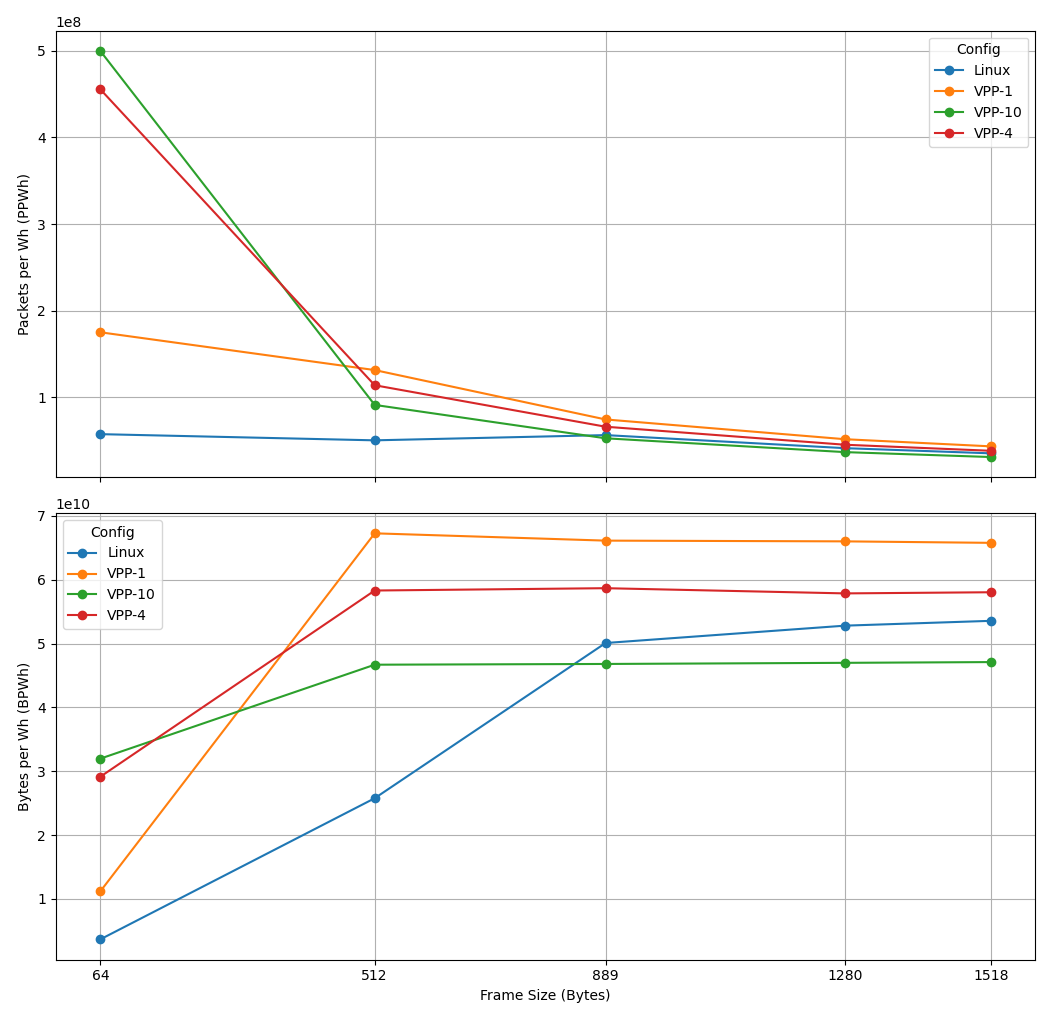
\includegraphics[width=\linewidth]{images/consumption-25g.png}
    \caption{Energy efficiency per delivered data in one-way 25\,Gbit/s.}
    \label{fig:25g}
\end{figure}


%-----------------------------------
\subsubsection{40 Gbps Test Results}

The results of the 40Gbit/s test, summarized in Table\ref{tab:40udp:64B}, clearly show that all configurations struggled to process the traffic.
The performance was comparable to the 25~Gbit/s test with 64-byte frames, but with even higher packet loss rates -- with the Linux stack delivering less than 5\% of the packets.

%------------------------------------------------------
\begin{table}[h!]
\centering
\caption{Results of one-way 40 Gbit/s of 64-byte frames}
\begin{tabular}{|l|r|r|r|r|r|r|}
\hline
\multicolumn{1}{|c|}{\textbf{Config}} &
\multicolumn{1}{c|}{\textbf{Energy [Wh] }} &
\multicolumn{1}{c|}{\textbf{Pkt Loss [\%]}} &
\multicolumn{1}{c|}{\textbf{Avg Lat [$\mu$s]}} &
\multicolumn{1}{c|}{\textbf{Jitter [$\mu$s]}} \\
\hline 
VPP-1 & 5.60 & 89.53 & 576.00 & 6.50 \\
VPP-4 & 6.57 & 67.54 & 195.70 & 6.57 \\
VPP-10 & 8.12 & 54.38 & 152.05 & 9.20 \\
Linux & 7.34 & 95.43 & 5629.05 & 550.30 \\
\hline
\end{tabular}
\label{tab:40udp:64B}
\end{table}

As the results in Table~\ref{tab:40udp:512B} suggest, only the VPP-1 and Linux configurations were unable to deliver all data,
while VPP-4 and VPP-10 showed significant improvements in latency.
The average latency of the Linux stack increased, which may be attributed to a larger number of packets being successfully delivered.

%------------------------------------------------------
\begin{table}[h!]
\centering
\caption{Results of one-way 40 Gbit/s of 512-byte frames}
\begin{tabular}{|l|r|r|r|r|r|r|}
\hline
\multicolumn{1}{|c|}{\textbf{Config}} &
\multicolumn{1}{c|}{\textbf{Energy [Wh] }} &
\multicolumn{1}{c|}{\textbf{Pkt Loss [\%]}} &
\multicolumn{1}{c|}{\textbf{Avg Lat [$\mu$s]}} &
\multicolumn{1}{c|}{\textbf{Jitter [$\mu$s]}} \\
\hline 
VPP-1 & 5.82 & 35.26 & 292.45 & 122.15 \\
VPP-4 & 6.56 & 0.00 & 28.80 & 9.90 \\
VPP-10 & 8.00 & 0.00 & 35.45 & 14.35 \\
Linux & TODO &  &  &  \\
\hline
\end{tabular}
\label{tab:40udp:512B}
\end{table}

In the 889-byte frame test, the results for VPP-4 and VPP-10 remained consistent with the previous experiment.
VPP-1 was almost able to handle the full traffic, while the Linux stack managed to process only about half of the data -- and did so with extremely high latency.
The results are summarized in Table~\ref{tab:40udp:889B}.

%------------------------------------------------------
\begin{table}[h!]
\centering
\caption{Results of one-way 40 Gbit/s of 889-byte frames}
\begin{tabular}{|l|r|r|r|r|r|r|}
\hline
\multicolumn{1}{|c|}{\textbf{Config}} &
\multicolumn{1}{c|}{\textbf{Energy [Wh] }} &
\multicolumn{1}{c|}{\textbf{Pkt Loss [\%]}} &
\multicolumn{1}{c|}{\textbf{Avg Lat [$\mu$s]}} &
\multicolumn{1}{c|}{\textbf{Jitter [$\mu$s]}} \\
\hline 
VPP-1 & 5.77 & 3.85 & 203.05 & 25.2 \\
VPP-4 & 6.54 & 0.00 & 32.55 & 13.75 \\
VPP-10 & 8.00 & 0.00 & 33.60 & 18.50 \\
Linux & 7.63 & 49.85 & 7222.80 & 315.40 \\
\hline
\end{tabular}
\label{tab:40udp:889B}
\end{table}

As the data in Table~\ref{tab:40udp:1280B} suggest, all VPP configurations performed similarly to the corresponding 25~Gbit/s test,
with the exception of VPP-1, which showed higher latency likely due to the increased traffic load.
The Linux stack was almost able to process all data, showing a significant improvement compared to the 889-byte frame test.

%------------------------------------------------------
\begin{table}[h!]
\centering
\caption{Results of one-way 40 Gbit/s of 1280-byte frames}
\begin{tabular}{|l|r|r|r|r|r|r|}
\hline
\multicolumn{1}{|c|}{\textbf{Config}} &
\multicolumn{1}{c|}{\textbf{Energy [Wh] }} &
\multicolumn{1}{c|}{\textbf{Pkt Loss [\%]}} &
\multicolumn{1}{c|}{\textbf{Avg Lat [$\mu$s]}} &
\multicolumn{1}{c|}{\textbf{Jitter [$\mu$s]}} \\
\hline 
VPP-1 & 5.79 & 0.00 & 32.50 & 14.65 \\
VPP-4 & 6.40 & 0.00 & 33.95 & 14.35 \\
VPP-10 & 8.02 & 0.00 & 32.15 & 16.85 \\
Linux & 7.59 & 6.25 & 2830.95 & 104.1 \\
\hline
\end{tabular}
\label{tab:40udp:1280B}
\end{table}

The data in Table~\ref{tab:40udp:1518B} demonstrate that the VPP configurations returned results comparable to the 1280-byte frame test,
indicating that the architecture has already reached its efficiency limit under the tested conditions.
In contrast, the Linux stack benefited from the increased frame size, being able to almost deliver the full traffic volume with significantly reduced latency.

%------------------------------------------------------
\begin{table}[h!]
\centering
\caption{Results of one-way 40 Gbit/s of 1518-byte frames}
\begin{tabular}{|l|r|r|r|r|r|r|}
\hline
\multicolumn{1}{|c|}{\textbf{Config}} &
\multicolumn{1}{c|}{\textbf{Energy [Wh] }} &
\multicolumn{1}{c|}{\textbf{Pkt Loss [\%]}} &
\multicolumn{1}{c|}{\textbf{Avg Lat [$\mu$s]}} &
\multicolumn{1}{c|}{\textbf{Jitter [$\mu$s]}} \\
\hline 
VPP-1 & 5.83 & 0.00 & 30.35 & 15.75 \\
VPP-4 & 6.43 & 0.00 & 34.20 & 14.75 \\
VPP-10 & 8.02 & 0.00 & 33.30 & 14.80 \\
Linux & 7.36 & 0.08 & 195.05 & 122.05 \\
\hline
\end{tabular}
\label{tab:40udp:1518B}
\end{table}









